\section{Introduction}

This document is the Software Specification Requirement (SRS) of a website designed to help earthquake victims to acquire necessary information and give volunteers a chance to donate for helping earthquake victims. The website is called \afetbilgi developed by Middle East Technical University (METU) students and graduates.

\subsection{Purpose of the System}

\afetbilgi, direct translation to English is `disaster documentation', is an open source efforted project led by students from METU in Ankara, Turkiye. It aims to provide a clean, verified and properly classified information interface for earthquake victims and helpers alike in the aftermath of the unfortunate earthquake on the Februrary  6th, 2023 in Pazarcik, Turkiye. Not only that, but it offers quick information with the use of confirmed website links, maps and address tables along with the relevant contact details of organisations and helpers involved.

\subsection{Scope}

\afetbilgi was established to offer as much information as needed by users in three main categories:
\begin{itemize}
  \item People who are affected by the earthquake (the victims). 
  \item Individuals/Organisations who want to help and take part in other government/private efforted procedures in the affected areas.
  \item People from METU who verify and checked any presented links on the websites.
\end{itemize}


The website at its core is primarily responsible for providing tables and datasheets with website links to third-party organisations/contacts details of web places/physical locations which offer/collect help. As indicated here, these links are external and lead out to other websites(outside from \afetbilgi) whose efforts are verified by human resolves (METU students/helpers/site administrators) on the surface level using past experience.

Given how the world is connected with the use of the internet in addition to phones/televised communication, the project developers aim to create a website using these advantageous characteristics via a simple interface in multiple available languages to create fast and easy use of information with no additional and unneccesary obstacles. In areas with a lack of internet infrastructure which might have disturbed by the earthquake activities, the website can be distributed via printed out PDFs (shareable via common computers and mobiles as well in addtional to hand forwarded physical versions in the forms of leaflets and so on).

Lastly, \afetbilgi includes a map functionality if the victim/helper indeed has an internet connection. Any user can locate helper geolocations via terrain/road routes while also be able to quickly view extra details such as written addresses, contact phone details and previous reviews.

\subsection{System Overview}

\subsubsection{System Perspective}

\afetbilgi \cite{afetbilgi} is not a part of a larger system. It is a standalone and open source efforted website to verify important information in the fight against the 6 February 2023 Pazarcik Earthquake and to deliver it to both disaster victims and those who want to help in an understandable, concise manner in multiple languages.

This information is presented in either the form of legible tables with 3rd party governmental and private links or an interactable method via a map view interface. If deemed necessary, admin and maintainers can make changes to display newly created or edited data and upload it to the system upon any complains or suggestion they may get on their contact details.

\begin{figure}[H]
  \centering
  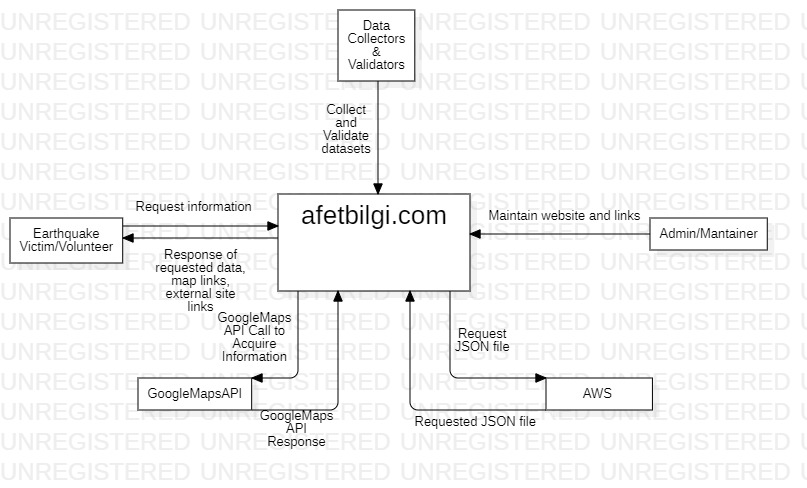
\includegraphics[width=\textwidth]{img/context-diagram.jpg}
  \caption{Context Diagram for \afetbilgi}
\end{figure}

\subsubsection{System Functions}

\subsubsection{Stakeholder Characteristics}

\subsubsection{Limitations}

\subsection{Definitions}
